\documentclass[11pt]{article}
\usepackage[T1]{fontenc}
\usepackage{lmodern,microtype,amsmath,amssymb,booktabs,graphicx,array}
\usepackage[margin=0.85in]{geometry}
\usepackage{xcolor,enumitem,pdfpages,xurl}
\definecolor{ink}{HTML}{18384A}
\definecolor{accent}{HTML}{287D89}
\usepackage[colorlinks=true,linkcolor=accent,urlcolor=accent,citecolor=accent]{hyperref}
\hypersetup{
 pdftitle={Three extensions of the ProveIt research program},
 pdfauthor={Research prepared for Vladimir Reshetnikov},
 pdfsubject={Positive filters, finite-field detection, and sharp integral Gram determinants}
}
\setlist{itemsep=4pt,topsep=5pt,leftmargin=*}
\setlength{\parskip}{5pt}
\setlength{\parindent}{0pt}
\newcommand{\F}{\mathbb F}
\newcommand{\R}{\mathbb R}
\newcommand{\Z}{\mathbb Z}
\newcommand{\E}{\mathbb E}
\newcommand{\TV}{d_{\mathrm{TV}}}
\newcommand{\rank}{\operatorname{rank}}
\newcommand{\Pois}{\operatorname{Pois}}
\newcommand{\PsiStar}{\Psi_*}
\newcommand{\guideheading}[1]{\section*{\color{ink}#1}\addcontentsline{toc}{section}{#1}}
\begin{document}
\pdfbookmark[0]{Research guide}{guide}
{\color{accent}\large PROVEIT \quad / \quad RESEARCH EXTENSIONS}\par
\vspace{9pt}
{\color{ink}\Huge\bfseries Three extensions of the\\[3pt] ProveIt research program}\par
\vspace{8pt}
{\large Sharp Gram determinants, optimal positive filters,\\
and two scales of finite-field detection}\par
\vspace{10pt}
Research prepared for Vladimir Reshetnikov \hfill 27 November 2026

{\color{accent}\rule{\linewidth}{1pt}}

\guideheading{Results delivered}
This collection supplies three complete proofs, executable checks, and a source audit.
Each result extends a specific mechanism or open direction in the supplied GRH
research program. All three theorems are unconditional.

\begin{enumerate}
\item \textbf{A sharp extremal law with an exact integer constraint.}
For rank-two integral matrices, the minimum normalized Gram determinant with
$n$ columns and $z$ zero pair minors is asymptotic to
\[
 \frac{n^6}{729\PsiStar^2z^2}
 \qquad\text{when }n=o(z),\quad z=o(n^2).
\]
The same constant holds for at most $z$ and for exactly $z$ zero minors.
A squared primitive-lattice potential determines $\PsiStar$, and a four-square
construction repairs the exact integer count.
\hyperref[paper:gram]{The complete proof is Paper I.}

\item \textbf{An exact local normal form for optimal positive filters.}
At every mirror configuration with strictly positive optimal masses, centered
polynomial coefficients give analytic coordinates through target collisions.
In suitable normal coordinates the shortest width is exactly
\[
 D=\frac{N\pi}{\kappa}+\|\eta\|^2.
\]
An explicit graph-energy formula gives the transverse Hessian.
\hyperref[paper:filters]{The complete proof is Paper II.}

\item \textbf{Two distinct transitions in a finite-field observation model.}
The exact finite likelihood uses only four matrix statistics. When $a=d-c$
nonzero anchors are observed through a complete bipartite pairing matrix,
dependence first becomes detectable near $m=a$, reaches a plateau, and
has a second Poisson transition near $m=q^d$.
\hyperref[paper:detection]{The complete proof is Paper III.}
\end{enumerate}

\textbf{Scope of the outcome.}
These proofs advance concrete open directions in the repository. They do not
establish a prominent classical conjecture. The source and related literature
were checked for overlap, but historical priority has not been exhaustively
certified. The proofs are written mathematical arguments with symbolic and
finite checks; they have not been formalized in Lean.

\textbf{Source snapshot.}
All comparisons use commit
\path{cfab41369737c66ae520d179419509eb719367cd}.
The source README distinguishes unconditional results, GRH consequences, and
reductions with remaining open estimates \cite{repo}. None of the three proofs
here invokes RH or GRH.

\newpage
\guideheading{I. A sharp Gram-determinant law}
Let $A=[v_1\ \cdots\ v_n]\in\Z^{2\times n}$ have rank two. Columns are indexed;
repeated, opposite, and zero columns are allowed. Define
\[
 D(A)=\gcd_{i<j}|\det(v_i,v_j)|,\qquad
 G(A)=\frac{\det(AA^{\mathsf T})}{D(A)^2},
 \qquad
 z(A)=\#\{i<j:\det(v_i,v_j)=0\}.
\]
Let $E_{\le}(n,z)$ and $E_{=}(n,z)$ minimize $G(A)$ under $z(A)\le z$ and
$z(A)=z$, respectively.

\textbf{Theorem.}
For every integer sequence with $z/n\to\infty$ and $z/n^2\to0$, the exact class
is eventually nonempty and
\[
 \boxed{E_{\le}(n,z)\sim E_{=}(n,z)
 \sim\frac{n^6}{729\PsiStar^2z^2}.}
\]
The constant is defined by the attained maximum
\[
 \PsiStar=\max_{T>0}
 \frac{16}{15T}\sum_{1\le j\le T}\frac{\varphi(j)}j
 \left(1-\frac{j^2}{T^2}\right)^{5/2}.
\]
This is an exact variational definition, not a numerical fit. The proof shows
$\Psi(T)\to1/\pi$ as $T\to\infty$ and certifies
\[
 0.318394611593156<\Psi(32/3)<0.318394611593166,
\]
which in particular is greater than $1/\pi$ and forces a finite maximizer.

\textbf{Why the scale changes.}
Normalize the generated column lattice, then replace each nonzero column by a
primitive vector in its direction. If the multiplicities are $m_v$ and there
are $k$ zero columns, then
\[
 \sum_v m_v^2=n+2z(A)-2kn+k^2\le Q:=n+2z.
\]
An area-preserving change of coordinates makes the Gram matrix isotropic.
Its total squared-length energy is then $2\sqrt{G(A)}$. For every radius $R$,
Cauchy--Schwarz bounds that energy below by
\[
 (n-k)R^2-
 \sqrt{Q\sum_v(R^2-|v|^2)_+^2}.
\]
Uniform primitive-lattice counting gives
\[
 \sum_v(R^2-|v|^2)_+^2
 =R^6\Psi(aR)+O(R^5\log(2R)),
\]
even for arbitrarily thin determinant-one lattices. Optimizing $R$ gives
$G(A)\ge(1-o(1))4n^6/(729\PsiStar^2Q^2)$.

\textbf{Why the lower bound is attained.}
At a maximizing aspect ratio, choose multiplicities proportional to
$(R^2-|v|^2)_+$. These parabolic weights saturate the quadratic budget and
the energy bound asymptotically. Rounding has lower-order cost.
Reserve eight distinct directions in four pairs with multiplicities
$M+x_j$ and $M-x_j$. They add exactly
\[
 4M(M-1)+\sum_{j=1}^4x_j^2
\]
zero minors while using exactly $8M$ columns. Lagrange's four-square theorem
therefore enforces the desired integer count with negligible energy.

\textbf{Interpretation and limit.}
If $z$ has order $n^{1+\alpha}$, $0<\alpha<1$, the optimal determinant has
order $n^{4-2\alpha}$. This extends the source's generic primitive-direction
method to substantial multiplicity. It does not determine fixed-$z$ asymptotics.
The numerical suggestion $\PsiStar\approx0.3183946273$ is explicitly
uncertified as a global maximum; neither uniqueness nor a ten-row
classification is asserted.

\newpage
\guideheading{II. Geometry of shortest positive filters}
A positive filter is a compactly supported probability measure $\mu$ on $\R$.
It cancels targets $s_1,\dots,s_N$ when its bilateral Laplace transform
\[
 F_\mu(s)=\int e^{st}\,d\mu(t)
\]
vanishes there, with repeated targets specifying derivative vanishing.
Let $D$ be the least support diameter.

\textbf{Local theorem at every positive equality configuration.}
Remove the common real mean by exponential tilting, set $h=\pi/\kappa$, and
write the centered target polynomial as
\[
 P_c(y)=y^N+\sum_{r=2}^N c_ry^{N-r}.
\]
At a mirror base, all $c_r$ are real. Assume every root $y_j$ lies in
$|\operatorname{Im}y|<\kappa$ and every coefficient of
\[
 A(z)=\prod_{j=1}^N(z+e^{hy_j})=\sum_{k=0}^N a_kz^k
\]
is strictly positive. In a coefficient neighborhood of this base:
\begin{itemize}
\item The global minimizer is unique up to translation and has exactly $N+1$
positive atoms, with analytic nodes and weights.
\item The width is analytic even when targets collide or split, and
\[
 C_1\|\operatorname{Im}c\|^2
 \le D(c)-Nh
 \le C_2\|\operatorname{Im}c\|^2.
\]
\item Its Hessian is positive definite transverse to the real-coefficient
locus, has exactly that tangent space as its kernel, and an analytic change
of normal coordinates gives $D(c)=Nh+\|\eta\|^2$.
\end{itemize}

\textbf{Explicit curvature.}
For $P_\epsilon=P_0+i\epsilon V$, $\deg V\le N-2$, write the node derivatives
as $\sigma_k$. Then
\[
 D=Nh+\epsilon^2 Q(V)+O(\epsilon^3),\qquad
 Q(V)=\frac1h\sum_{j<k}a_ja_k(\sigma_j-\sigma_k)^2
 \int_0^\infty\frac{z^{j+k-1}}{A(z)^2}\,dz .
\]
Confluent Hermite interpolation identifies $V$ with the internal node
velocities. A persistent dual certificate proves global optimality, while
an exact strip-integral deficit gives this positive curvature formula.

\textbf{A concrete interaction law.}
For two nearby modes $s_\pm=\pm\beta+i(\kappa\pm\delta)$,
\[
 D=\frac{2\pi}{\kappa}
 +\frac{4\pi^3}{3\kappa^5}\beta^2\delta^2
 \left[1+O\!\left(\frac{\beta^2+\delta^2}{\kappa^2}\right)\right].
\]
Pure damping or pure frequency splitting has no local cost; their interaction
has a positive quartic cost.

\textbf{Further conclusions and scope.}
Paper II also proves $D\ge N^2\pi/\sum_j\operatorname{Im}s_j$ for arbitrary
upper-half-plane targets with unrelated damping. An exact cubic example
shows that mixed Hessian entries can be negative. The normal form is local
for fixed degree, requires strictly positive base masses, and does not
cover zero-mass support transitions.

\newpage
\guideheading{III. Two scales of finite-field detection}
Fix a prime power $q$, a dimension $d$, and $N=q^d$. Sample $a$ anchors
$X_i$ and $m$ probes $Z_j$ independently and uniformly from
$\F_q^d\setminus\{0\}$. Observe $Y_{ij}=B(X_i,Z_j)$ for a nondegenerate
bilinear form $B$. Let $P$ be its law and $Q$ the independent-entry law
with the same one-entry marginal.

\textbf{Exact finite result.}
The complete likelihood ratio depends only on
\[
 \rank Y,\quad\#\{\text{zero rows}\},\quad
 \#\{\text{zero columns}\},\quad\#\{\text{zero entries}\}.
\]
Paper III gives the exact Gaussian-binomial inclusion-exclusion formula.
An optimal test may therefore be chosen using only these four statistics.

\textbf{Fixed codimension.}
Put $a=d-c$ for a fixed $c\ge0$, and
\[
 \alpha_c=\prod_{i=c+1}^{\infty}(1-q^{-i}).
\]
A classical random-matrix rank transition occurs near $m=a$. In the range
$m-a\to\infty$, $m=o(q^d)$, total variation converges to $1-\alpha_c$.
If $m/N\to\lambda<\infty$ while $m-a\to\infty$, a second transition has
the exact limit
\[
 \boxed{\TV(P,Q)\longrightarrow
 1-\E_{Z\sim\Pois(\lambda q^c)}
 \min\{1,\alpha_ce^\lambda(1-q^{-c})^Z\}.}
\]
The limiting alternative has a rank-deficient flag of mass $1-\alpha_c$;
conditional on its complement, the zero-column count is
$\Pois(\lambda(q^c-1))$. Under the null it is $\Pois(\lambda q^c)$.
These two statistics retain asymptotically all testing information.

\begin{center}
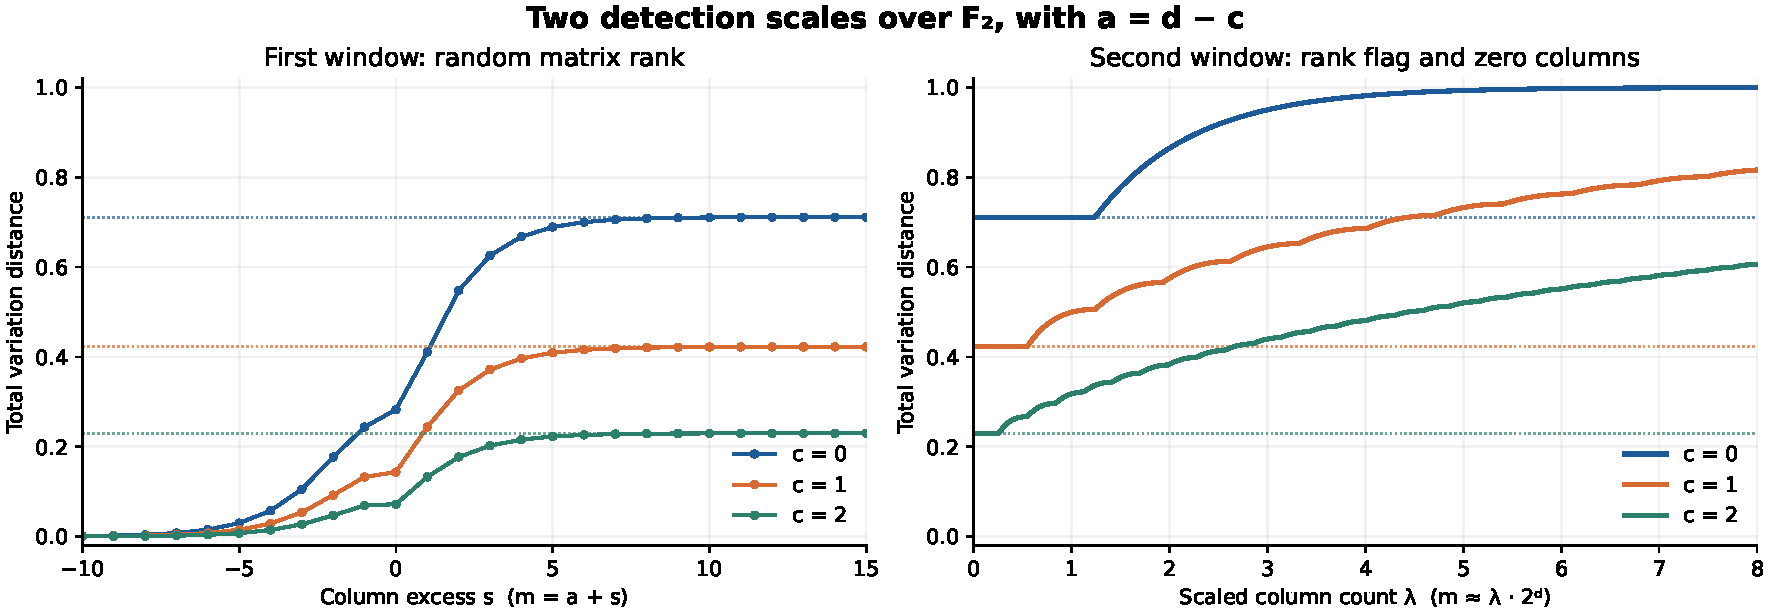
\includegraphics[width=\linewidth]{papers/bilinear_detection/two_scales.pdf}
\end{center}
\vspace{-8pt}
{\small Curves evaluate the proved limiting formulas; they are not simulated data.
The horizontal axes describe two different asymptotic windows.}

For $q=2,c=0$, the second profile simplifies to
\[
 \max\{0.7112119049133976\ldots,\;1-e^{-\lambda}\}.
\]
It leaves its plateau at $\lambda=1.242062094812415\ldots$.
For $c\ge1$, the corners occur exactly at
$-\log\alpha_c+j\log(1/(1-q^{-c}))$, $j=0,1,\dots$.

\textbf{Growing codimension.}
If $d-a\to\infty$ and
$m(q^a-1-a(q-1))/q^{2d}\to\tau$, then the limit is
$2\Phi(\sqrt\tau/2)-1$. This makes the source's fixed-anchor Gaussian
theorem uniform in growing anchor number and explains the transition
to the fixed-codimension experiment.

\newpage
\guideheading{IV. Source relationship and proof evidence}
The source article develops many transfers from its RH/GRH program. The
three contributions here use its unconditional mechanisms:

\begin{center}\small
\begin{tabular}{@{}>{\raggedright\arraybackslash}p{0.17\linewidth}>{\raggedright\arraybackslash}p{0.35\linewidth}>{\raggedright\arraybackslash}p{0.40\linewidth}@{}}
\toprule
Strand & Inherited mechanism & Addition in this collection\\
\midrule
Gram & Primitive lattice directions; generic rank-two potential &
Squared potential; quadratic multiplicity budget; sharp growing-$z$ law;
exact integer repair\\[5pt]
Filters & Reflection certificate; strip identity; special Hessians &
General positive mirror base; coefficients through collisions;
positive normal form; changing mixed signs\\[5pt]
Detection & Independent-anchor decomposition; fixed-anchor critical law &
Exact constrained likelihood; retained dependent-anchor mass;
rank/Poisson experiment; uniform Gaussian regime\\
\bottomrule
\end{tabular}
\end{center}

Precise source labels and distinctions from relevant incoming reports appear
in \path{SOURCE_AUDIT.md}. The Gram result addresses a growing-degeneracy
part of \texttt{src:q:gram}; the filter theorem addresses the sign and
degeneracy part of \texttt{fil:sec:open}, item 2; the detection theorem
addresses a growing complete-bipartite regime of
\texttt{spn:q:dependence}. None is presented as solving the whole associated
open-question list.

\textbf{Computational evidence included.}
\begin{itemize}
\item Exact symbolic interpolation and rational integration for the filter
Hessian, plus twelve independent nonlinear solves at 80-digit precision.
The nine cubic moment residuals are below $10^{-60}$.
\item Nine exhaustive finite-field cases: 440,836 latent assignments and
87,149 possible observed matrices, including zero-probability matrices.
Eighteen additional exact column calculations check the chi-square formula.
\item A separately implemented conditional-count check covers 53,114,420
latent assignments by exact aggregation, checking all 818 possible matrices
across six cases.
\item A rational certificate for the Gram potential, five exact weighted
matrix examples, and an exact four-square correction. The largest example
represents 47,765,579 indexed columns compactly. The correction example has
18,048 columns and exactly 1,140,772 zero minors.
\end{itemize}

\textbf{Proof review.}
Separate reasoning passes checked the confluent Jacobian, persistent global
certificate, zero counting, and Hessian differentiation in the filter
paper; finite likelihood normalization, defective Poisson mass, and
uniform variance estimates in the detection paper; and the uniform
lattice error, sharp constants, rounding, and integer repair in the Gram
paper. These are internal checks, not external peer review. The
mathematical arguments do not rely on the finite checks as proofs.

\textbf{Limitations retained.}
The exact Gram variational constant does not imply a certified unique
maximizer. The filter normal form is local at a strictly positive base and
uses coefficient coordinates. The detection theorem concerns the specified
sampling model on complete bipartite graphs. General support transitions,
fixed-$z$ sharp Gram laws, and general overlapping-cycle observation graphs
remain open. No named classical conjecture is claimed resolved.

\newpage
\guideheading{V. Reproduction and related work}
Run the following from the unpacked archive:
\begin{verbatim}
python3 -m pip install -r requirements.txt
python3 verify_all.py
python3 build.py
\end{verbatim}
The build compiles each paper and then this collected report. Add
\texttt{--figures} to regenerate the detection diagram. No network access
or upstream proof checkout is needed once the dependencies are installed.
The exact Gram and primary finite-field checkers use Python's standard
library; the remaining checks use NumPy, SymPy, mpmath, and Matplotlib.
Version information and run records are included.

The archive contains every paper's \texttt{.tex} and \texttt{.pdf}, code,
JSON results, profile data, figures, source hashes, and build instructions.
The standalone PDFs retain their internal references. This collected
version preserves their printed page numbers; the PDF bookmarks locate
each paper.

\textbf{Related literature.}
The filter zero-counting context includes Eremenko--Fryntov's work on
Obrechkoff's inequality \cite{ef}, and positive input shaping has an
established control-theory literature \cite{input}. The first detection
scale uses classical finite-field rank distributions \cite{fg}; graph-masked
real Wishart models provide a related but distinct dependence problem
\cite{bbh}. The closest inspected lattice-extremal work concerns sums of
absolute determinants \cite{bt} or bounds on the largest minor \cite{ks},
rather than our multiplicity-constrained sum of squared normalized minors.
These comparisons support a scoped contribution claim, not an exhaustive
historical priority certificate.

\begingroup\small
\begin{thebibliography}{9}
\bibitem{repo}
V. Reshetnikov, \emph{ProveIt}, commit
\path{cfab41369737c66ae520d179419509eb719367cd}, especially
\path{Article/README.md} and \path{Article/sections/src.tex},
\path{fil.tex}, and \path{spn.tex}.
\url{https://github.com/VladimirReshetnikov/ProveIt/tree/cfab41369737c66ae520d179419509eb719367cd/Analysis/GeneralizedRiemannHypothesis}.
\bibitem{ef}
A. Eremenko and A. Fryntov, \emph{Remarks on the Obrechkoff inequality},
Proc. Amer. Math. Soc. 144 (2016), 703--707.
\url{https://arxiv.org/abs/1409.4849}.
\bibitem{input}
W. Singhose, E. Crain, and W. Seering, \emph{Convolved and simultaneous
two-mode input shapers}, IEE Proc.--Control Theory Appl. 144 (1997), 515--520.
\url{https://doi.org/10.1049/ip-cta:19971439}.
\bibitem{fg}
J. Fulman and L. Goldstein, \emph{Stein's method and the rank distribution
of random matrices over finite fields}, Ann. Probab. 43 (2015), 1274--1314.
\url{https://doi.org/10.1214/13-AOP889}.
\bibitem{bbh}
M. Brennan, G. Bresler, and B. Huang, \emph{De Finetti-style results for
Wishart matrices: combinatorial structure and phase transitions},
arXiv:2103.14011 (2021). \url{https://arxiv.org/abs/2103.14011}.
\bibitem{bt}
I. B\'ar\'any and N. Tokushige, \emph{The minimum area of convex lattice
$n$-gons}, Combinatorica 24 (2004), 171--185.
\url{https://www.renyi.hu/~barany/cikkek/94.pdf}.
\bibitem{ks}
B. Kriepke and M. Schymura, \emph{On generic $\Delta$-modular integer
matrices with two rows}, SIAM J. Discrete Math. 40 (2026), 1342--1368.
\url{https://doi.org/10.1137/25M1745878}.
\end{thebibliography}
\endgroup

\clearpage
\hypersetup{pageanchor=false}
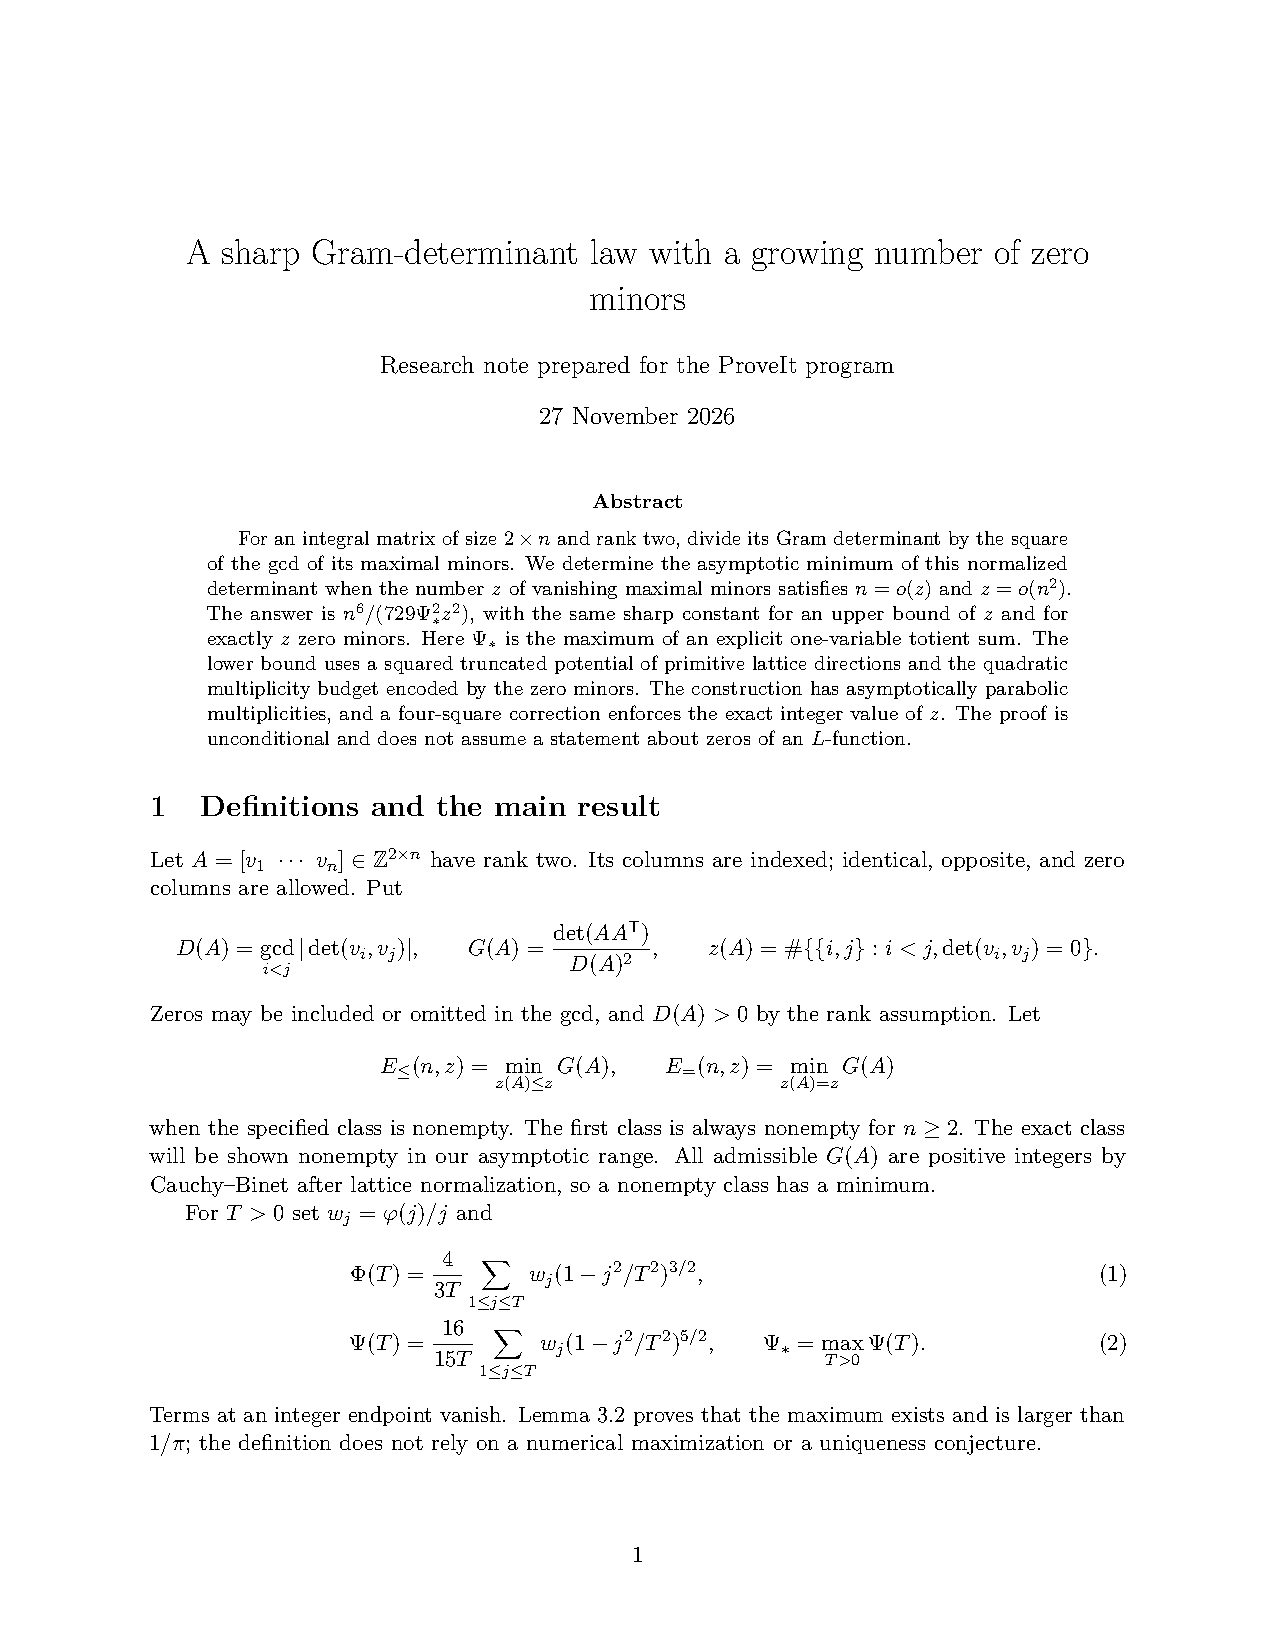
\includepdf[pages=-,pagecommand={\thispagestyle{empty}},
 addtotoc={1,section,1,Paper I. Sharp Gram determinants,paper:gram}]
 {papers/gram_determinants/gram_determinants.pdf}
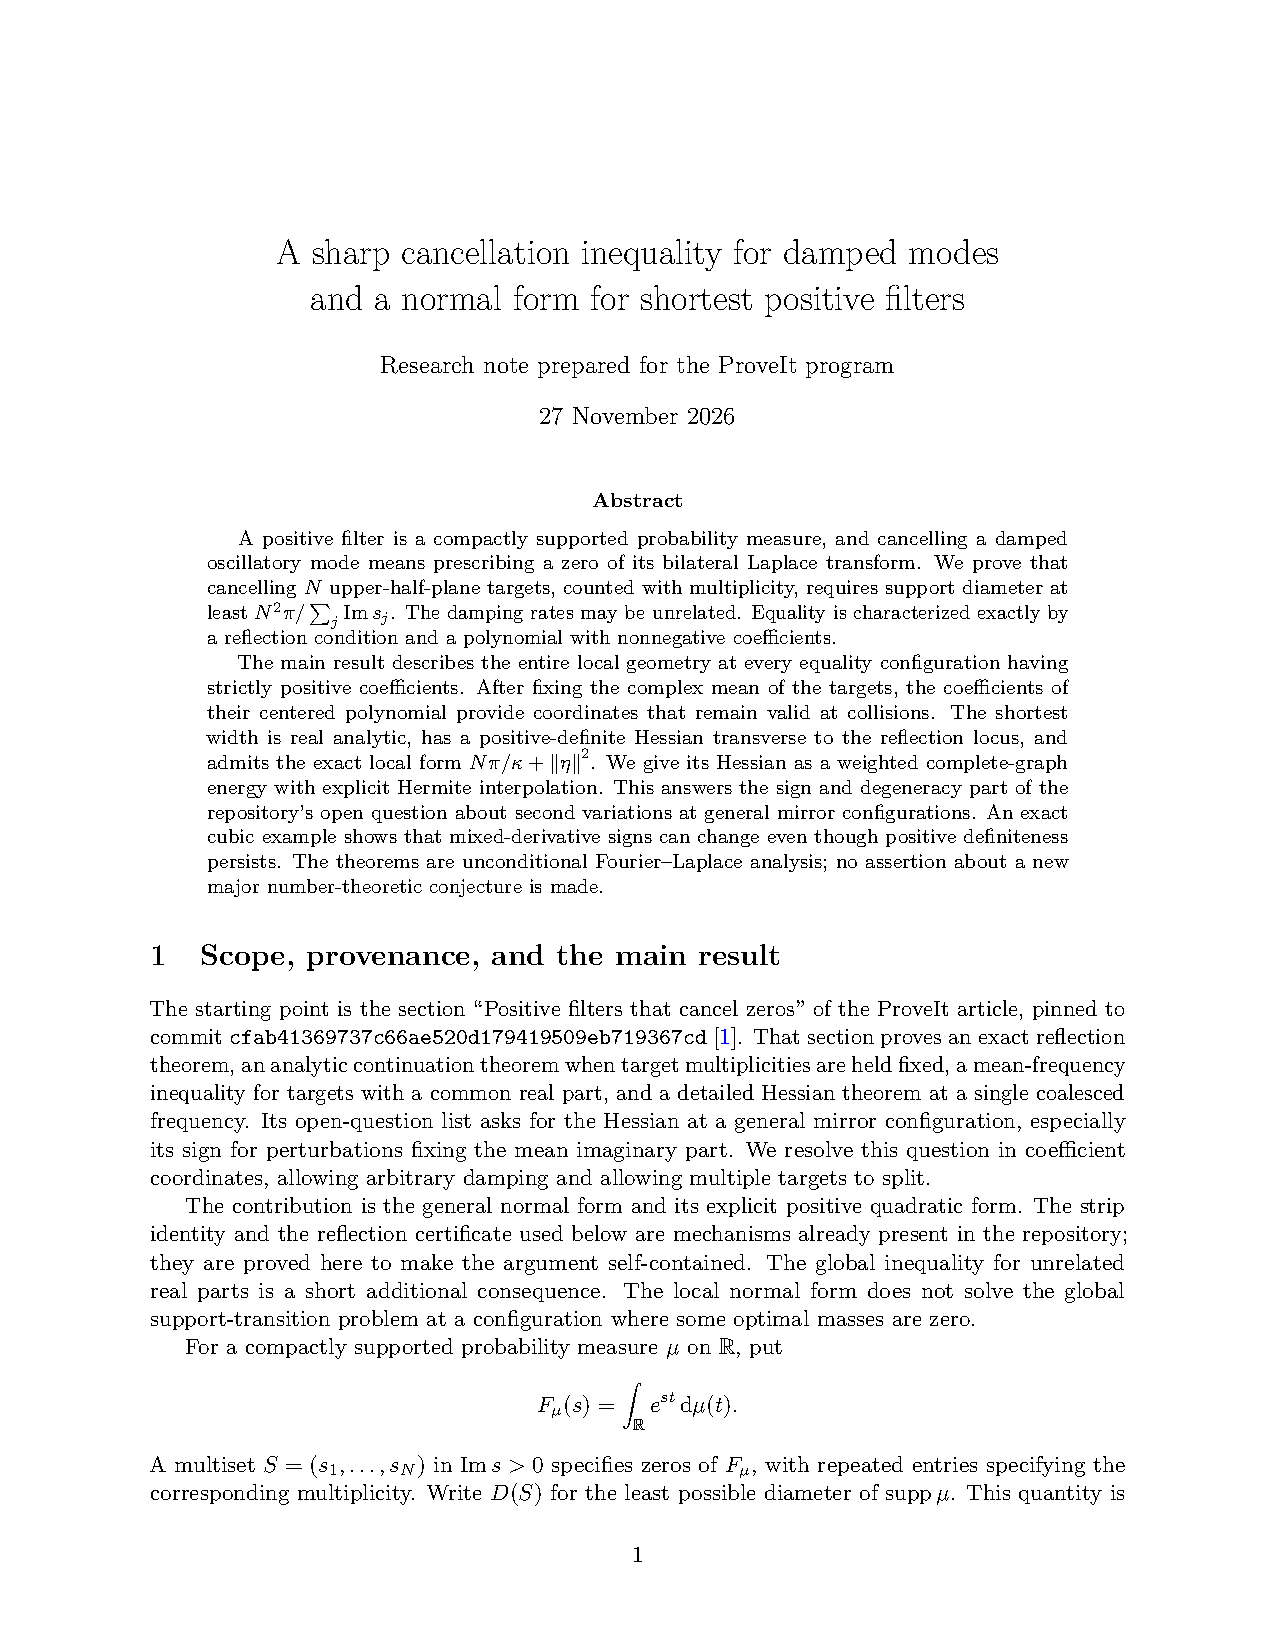
\includepdf[pages=-,pagecommand={\thispagestyle{empty}},
 addtotoc={1,section,1,Paper II. Shortest positive filters,paper:filters}]
 {papers/positive_filters/positive_filters.pdf}
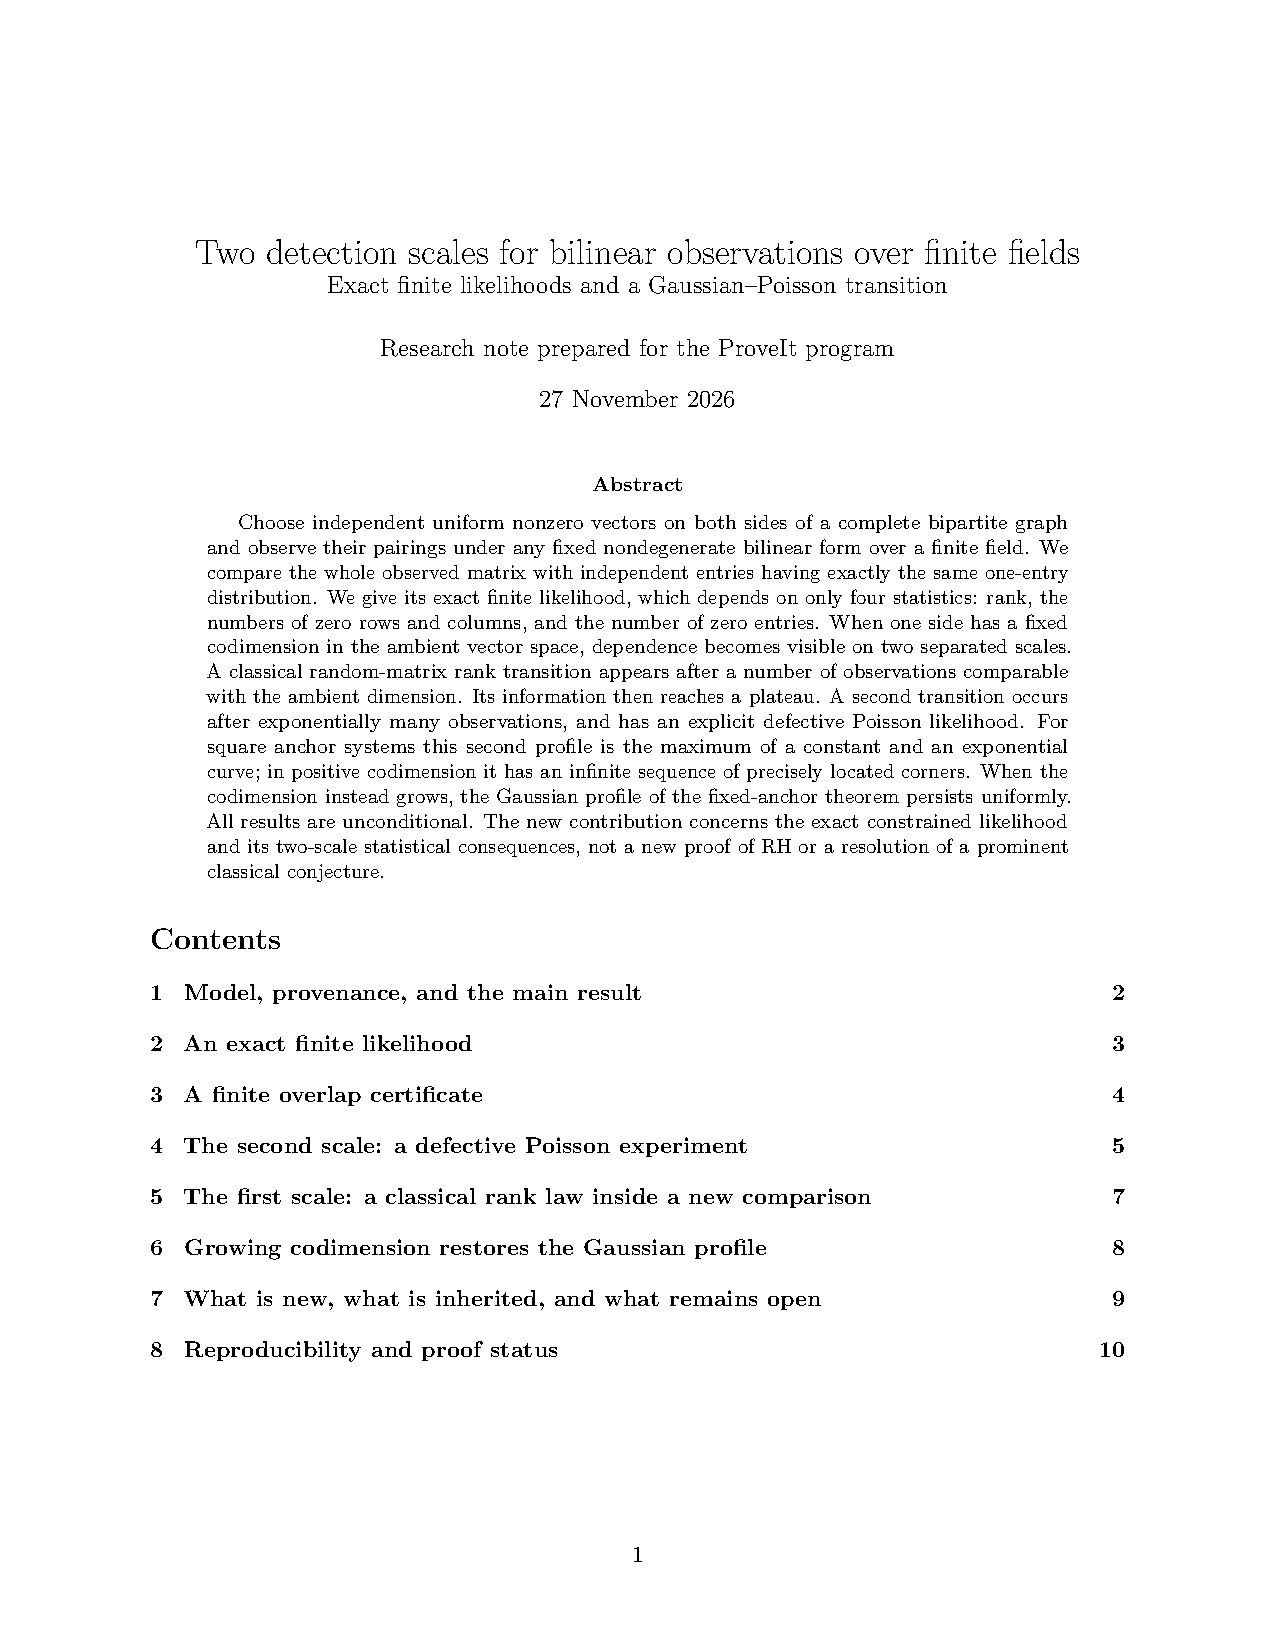
\includepdf[pages=-,pagecommand={\thispagestyle{empty}},
 addtotoc={1,section,1,Paper III. Two detection scales,paper:detection}]
 {papers/bilinear_detection/bilinear_detection.pdf}
\end{document}
